\documentclass[a4paper]{article}
\usepackage{graphicx} %Required for diagrams
\usepackage[bookmarks=true]{hyperref}
\usepackage{bookmark}%Required to do pdf bookmarking
\usepackage[margin=1.2in]{geometry}
\usepackage{float}
\usepackage{caption}
\usepackage{hyperref}%Required for referencing website pages
\usepackage[english]{babel}

\usepackage{graphicx}
\usepackage{dcolumn}
\usepackage[table]{xcolor}

\title{Sprint Eight Report}
\author{Baobab Team}

\begin{document}
\newpage

\begin{titlepage}

\begin{center}


\includegraphics[width=400px]{pictures/logo.jpg}
\vspace{0.5 cm}
\begin{flushright} \large
\begin{tabular}{lr}
\vspace{1 cm}
\LARGE\textbf{Document:}Sprint Report 6\\

\vspace{1 cm}
\LARGE\textbf{Project:} Group Chat For Linphone (Agile DO-178)\\
\vspace{1 cm}
\LARGE\textbf{Advisor:} Kobus Coetzee\\
\vspace{1 cm}
\LARGE\textbf{Sponsors:} Nanoteq \& Department of Computer Science, UP\\
\vspace{1 cm}
\LARGE\textbf{Date: }\today\\
\end{tabular}
\end{flushright}

\centering 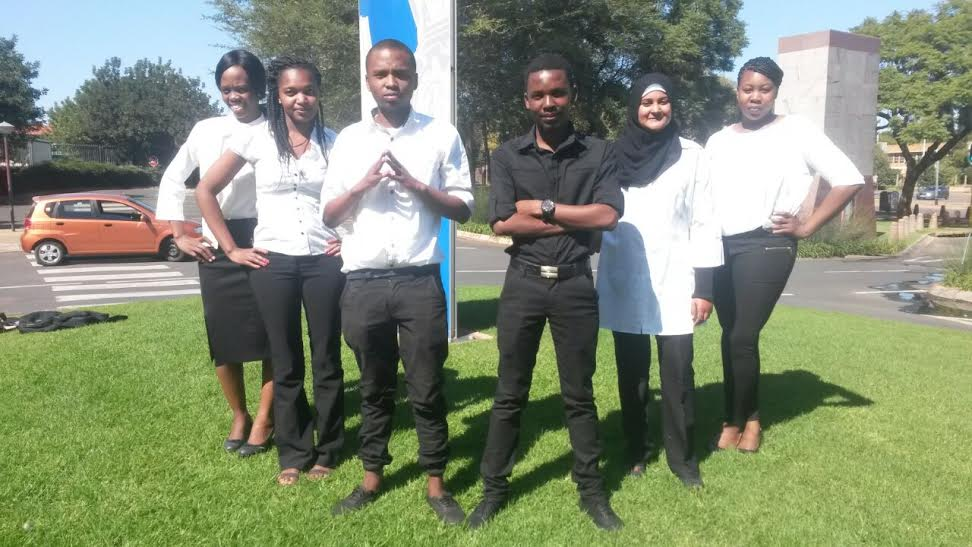
\includegraphics[width=350px]{pictures/Team.jpg}

Patience Mtsweni, Lerato Molokomme, Tsepo Ntsaba, Mpedi Mello, Lutfiyya Razak, Ephiphania Munava\\


\end{center}
\end{titlepage}
\newpage

\section{Product Backlog}

\begin{figure}[H]
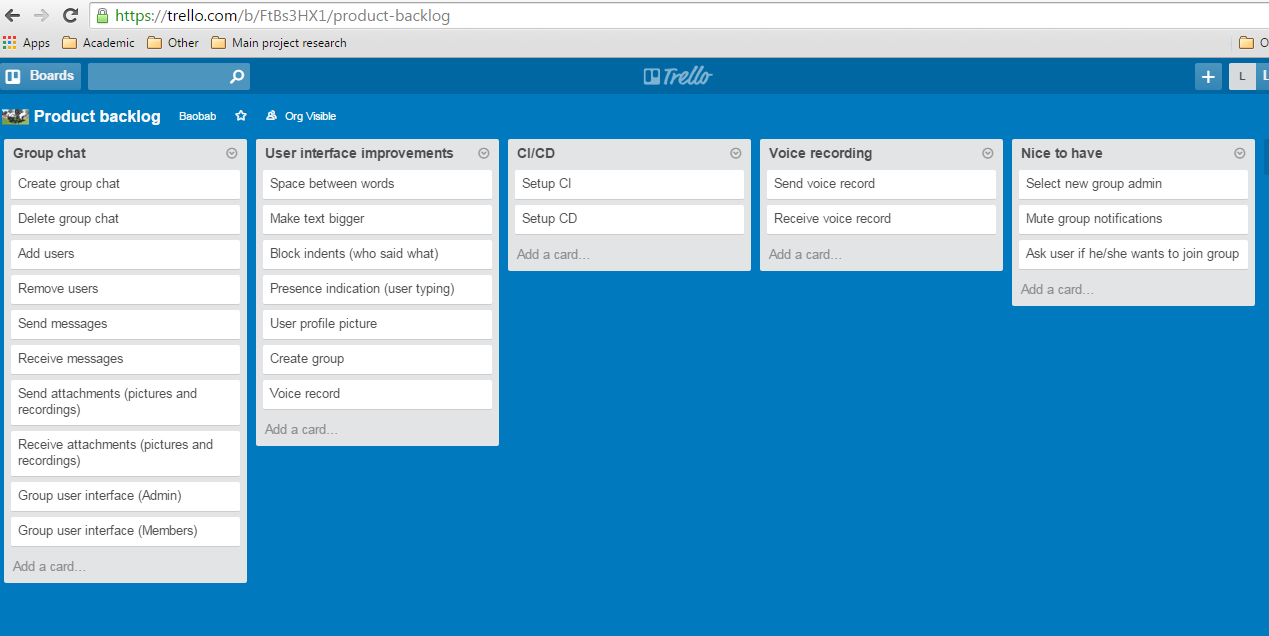
\includegraphics[width=1\linewidth]{./pictures/backlog.jpg}\\
\caption{\label{fig:Product Backlog}Product Backlog}
\end{figure}

\href{https://trello.com/b/FtBs3HX1}{Click-able link to Product Backlog on Trello}


\section{Sprint Review}

\subsection{Participants}

\setlength{\arrayrulewidth}{0.5mm}
\setlength{\tabcolsep}{12pt}
\renewcommand{\arraystretch}{2} 
\begin{tabular}{ |p{3cm}|p{3cm}|p{3cm}|  }
\hline
\rowcolor{lightgray}\multicolumn{2}{|c|}{Scrum User Roles} \\
\hline
Role & Name\\
\hline
Scrum master  & Potego Mello\\ \hline 
Client representative  & Patience Mtsweni\\ \hline 
UX developer  & Lutfiyya Razak and Lerato Molokomme\\ \hline 
Backend developer  & Ephiphania Munava and Potego Mello\\ \hline 
Crypto developer  & Tsepo Ntsaba \\ \hline 
CI / CD support  & Patience Mtsweni \\ 
\hline
\end{tabular}

\subsection{Sprint Summary}
\setlength{\arrayrulewidth}{0.5mm}
\setlength{\tabcolsep}{12pt}
\renewcommand{\arraystretch}{2} 
\begin{tabular}{ |p{2.5cm}|p{2.5cm}|p{2.5cm} |p{2.5cm}| }
\hline
\rowcolor{lightgray}\multicolumn{4}{|c|}{Sprint Summary} \\
\hline
Sprint Number & Sprint & Start Date & End Date\\
\hline 
1 & Environment Setup & 23 June 2015 & 1 July 2015 \\
\hline
2 & CI Setup & 1 July 2015 & 12 July 2015 \\
\hline
3 & User Interface  and Create Group Chat & 13 July 2015 & 27 July 2015 \\
\hline
4 & Group Chat Implementation & 29 July 2015 & 16 August 2015 \\
\hline
5 & Group Chat Implementation & 17 July 2015 & 30 August 2015 \\
\hline
6 & Message Interactions and Encryption & 30 August 2015 & 13 September 2015 \\
\hline
7 & Group Administration and Encryption & 13 September 2015 & 27 September 2015 \\
\hline
8 & Group Administration and Encryption & 27 September 2015 & 11 October 2015 \\
\hline
\end{tabular}

\subsection{Software Architecture}
\textbf{Description: }We did not modify the software architecture. \\

\subsection{Sprint Summary}
\subsubsection{What we got done: }
\textbf{Description: }We did a review of the eight sprint and we discussed our next sprint(sprint nine). We discussed the user stories as well as our roles and what we expected to deliver. \\

\setlength{\arrayrulewidth}{0.5mm}
\setlength{\tabcolsep}{12pt}
\renewcommand{\arraystretch}{2} 
\begin{tabular}{ |p{2.5cm}|p{2.5cm}|p{2.5cm}|p{2.5cm}| p{2.5cm}| }
\hline
\rowcolor{lightgray} \multicolumn{5}{|c|}{Completed Work} \\
\hline
Date Complete & Implemented in production quality & Tested & Integrated & Documented \\
\hline
23 June 2015 & Yes & Product Backlog & Not Applicable & \href{https://trello.com/b/FtBs3HX1}{Click-able link to Product Backlog on Trello}\\ \hline
23 June 2015 & Yes & Environment Setup Sprint & Not Applicable & \href{https://trello.com/b/hBJF6EUd}{Click-able link to Sprint Backlog on Trello}\\ 
\hline
30 June 2015 & Yes & User Interface and CI Setup & Yes & \href{https://trello.com/b/hBJF6EUd}{Click-able link to Sprint Backlog on Trello}\\ 
\hline
13 August 2015 & Yes & Group Chat Implementation & Yes & \href{https://trello.com/b/hBJF6EUd}{Click-able link to Sprint Backlog on Trello}\\ 
\hline
30 August 2015 & Yes & Message Interactions and Encryption & Yes & \href{https://trello.com/b/hBJF6EUd}{Click-able link to Sprint Backlog on Trello}\\ 
\hline
13 September 2015 & Yes & Message Interactions and Encryption & Yes & \href{https://trello.com/b/hBJF6EUd}{Click-able link to Sprint Backlog on Trello}\\ 
\hline
30 September 2015 & Yes & Group Administration and Encryption & Yes & \href{https://trello.com/b/hBJF6EUd}{Click-able link to Sprint Backlog on Trello}\\ 
\hline
\end{tabular}

\subsection{What we plan to do next:}
\textbf{Description: }We implementing the following user stories:
\begin{enumerate} 
\item I can get help during the group creation process.
\item I can get information during the group creation process.
\item I can select a group name.
\item I can select a group icon.
\item I can encrypt messages with a fixed key.
\end{enumerate}

\setlength{\arrayrulewidth}{0.5mm}
\setlength{\tabcolsep}{12pt}
\renewcommand{\arraystretch}{2} 
\begin{tabular}{ |p{3cm}|p{3cm}|p{3cm}|p{3cm}|p{3cm}|  }
\hline
\rowcolor{lightgray}\multicolumn{4}{|c|}{Work to Complete} \\
\hline 
Date to begin & Task to implement: & Assigned To: & Date to complete\\
\hline
13 September 2015 & I can get help during the group creation process. & Lutfiyya(GUI) and  Potego(Back-End) & 30 September 2015\\ 
\hline
13 September 2015 & I can get information during the group creation process. & Lutfiyya(GUI) and Potego(Back-End) & 30 September 2015\\ 
\hline
13 September 2015 & I can select a group name. & Tsepo  & 30 September 2015\\ 
\hline
13 September 2015 & I can select a group icon. & Tsepo  & 30 September 2015\\ 
\hline
13 September 2015 & I can encrypt messages with a fixed key & Tsepo  & 30 September 2015\\ 
\hline
\end{tabular}

\end{document}